%%%%%%%%%%%%%%%%%%%%%%%%%%%%%%%%%%%%%%%%%%%%%%%%%%%%%%%%%%%%%%%%%%%%%%%%%%%%%%%%%%
\begin{frame}[fragile]\frametitle{}
\begin{center}
{\Large Overview of Large Language Models}
\end{center}
\end{frame}

%%%%%%%%%%%%%%%%%%%%%%%%%%%%%%%%%%%%%%%%%%%%%%%%%%%%%%%%%%%
\begin{frame}[fragile]\frametitle{What is a Language Models?}

\begin{itemize}
\item While typing SMS, have you seen it suggests next word?
\item While typing email, have you seen next few words are suggested?
\item How does it suggest? (suggestions are not random, right?)
\item In the past, for ``Lets go for a \ldots', if you have typed 'coffee' 15 times, 'movie' say 4 times, then it learns that. Machine/Statistical Learning.
\item Next time, when you type ``Lets go for a '', what will be suggested? why?
\item This is called Language Model. Predicting the next word. When done continuously, one after other, it spits sentence, called Generative Model.
\end{itemize}	

\begin{center}
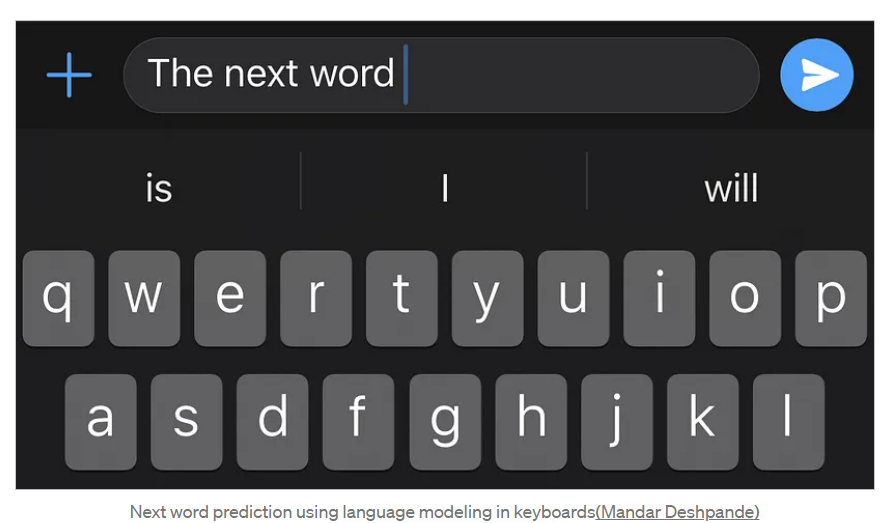
\includegraphics[width=0.6\linewidth,keepaspectratio]{chatgpt34}
\end{center}		

\end{frame}

%%%%%%%%%%%%%%%%%%%%%%%%%%%%%%%%%%%%%%%%%%%%%%%%%%%%%%%%%%%
\begin{frame}[fragile]\frametitle{Evolution of Language Models}

Language Models can be statistical (frequency based) or Machine/Deep Learning (supervised) based. Simple to complex.

\begin{center}
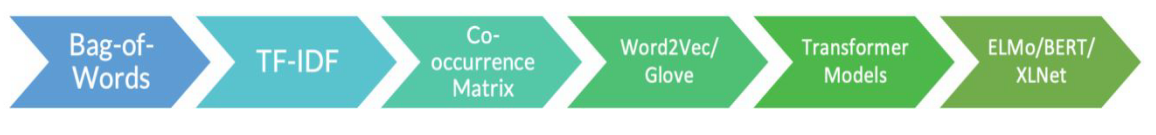
\includegraphics[width=\linewidth,keepaspectratio]{chatgpt30}
\end{center}				
{\tiny (Ref: Analytics Vidhya https://editor.analyticsvidhya.com/uploads/59483evolution\_of\_NLP.png)}

\end{frame}

%%%%%%%%%%%%%%%%%%%%%%%%%%%%%%%%%%%%%%%%%%%%%%%%%%%%%%%%%%%
\begin{frame}[fragile]\frametitle{Large Language Models - Comparison}

\begin{center}
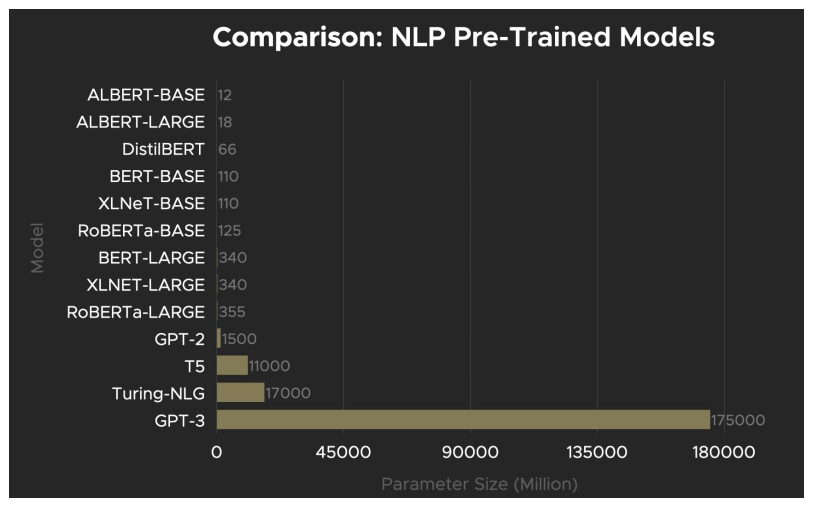
\includegraphics[width=\linewidth,keepaspectratio]{chatgpt31}
\end{center}				
{\tiny (Ref: Deus.ai https://www.deus.ai/post/gpt-3-what-is-all-the-excitement-about)}

\end{frame}


%%%%%%%%%%%%%%%%%%%%%%%%%%%%%%%%%%%%%%%%%%%%%%%%%%%%%%%%%%%
\begin{frame}[fragile]\frametitle{GPTs Training}

GPT: Generative Pre-trained Transformers

\begin{itemize}
% \item GPT-1 is trained in a self-supervised manner (learn to predict the next word in text data) and fine-tuned in a supervised learning manner. 
% \item GPT-2 is trained in a fully self supervised way, focusing on zero-shot transfer
% \item  GPT-3 is pre-trained in a self supervised manner exploring a bit more the few-shots fine-tuning.
\item GPT-1 is pre-trained on the BooksCorpus dataset, containing ~7000 books amounting to ~5GB of data
\item GPT-2 is pre-trained using the WebText dataset which is a more diverse set of internet data containing ~8M documents for about ~40 GB of data
\item GPT-3 uses an expanded version of the WebText dataset, two internet-based books corpora that are not disclosed and the English-language Wikipedia which constituted ~600 GB of data
\end{itemize}	 

\end{frame}

%%%%%%%%%%%%%%%%%%%%%%%%%%%%%%%%%%%%%%%%%%%%%%%%%%%%%%%%%%%
\begin{frame}[fragile]\frametitle{GPTs Training compared to human reading}

\begin{itemize}
% \item GPT-1 is trained in a self-supervised manner (learn to predict the next word in text data) and fine-tuned in a supervised learning manner. 
% \item GPT-2 is trained in a fully self supervised way, focusing on zero-shot transfer
% \item  GPT-3 is pre-trained in a self supervised manner exploring a bit more the few-shots fine-tuning.
\item GPT-3 was trained on 499B tokens; GPT-4, on 1.4T tokens.
\item In comparison, if you spent 12 hours a day reading for an entire lifetime (80 years) at average speed (250 words / minute), we would absorb 5.26B words (tokens).
\item That's a ratio of 100:1 between the training data used for GPT-3 and the amount of data that can ever be read by a human, and 260:1 for GPT-4.
\end{itemize}	 

\tiny{(Ref: LinkedIn post by Dr Jennifer Prendki)}

\end{frame}


%%%%%%%%%%%%%%%%%%%%%%%%%%%%%%%%%%%%%%%%%%%%%%%%%%%%%%%%%%%%%%%%%%%%%%%%%%%%%%%%%%
\begin{frame}[fragile]\frametitle{Other Use Cases}
	

\begin{itemize}
\item Image: the AI will generate a new image based on your prompt and the image provided.
\item Embeddings: turn input into a vector representation. It’s very useful when we need to compare the similarity between two texts.
\item Audio: turn audio into text.
\end{itemize}	 

{\tiny (Ref: Techy Stuff 1: Notes on Transformers, LLMs, and OpenAI - Bill)}
			
\end{frame}
